%%%%%%%%%%%%%%%%%%%%%%%%%%%%%%%%%%%%%%%%%
% Simple Sectioned Essay Template
% LaTeX Template
%
% This template has been downloaded from:
% http://www.latextemplates.com
%
% Note:
% The \lipsum[#] commands throughout this template generate dummy text
% to fill the template out. These commands should all be removed when 
% writing essay content.
%
%%%%%%%%%%%%%%%%%%%%%%%%%%%%%%%%%%%%%%%%%

%----------------------------------------------------------------------------------------
%	PACKAGES AND OTHER DOCUMENT CONFIGURATIONS
%----------------------------------------------------------------------------------------

%\documentclass[12pt]{article} % Default font size is 12pt, it can be changed here

%\usepackage{geometry} % Required to change the page size to A4
%\geometry{letterpaper} % Set the page size to be A4 as opposed to the default US Letter

%\usepackage{graphicx} % Required for including pictures

%\usepackage{listings} %Para comandos bash Linux

%\usepackage{float} % Allows putting an [H] in \begin{figure} to specify the exact location of the figure
%\usepackage{wrapfig} % Allows in-line images such as the example fish picture

%\usepackage{color} %textos de colores

%\usepackage[spanish]{babel}

%\usepackage[utf8]{inputenc} %Uso de acentos directamente

%\usepackage{hyperref}

%\linespread{1.2} % Line spacing

%\setlength\parindent{0pt} % Uncomment to remove all indentation from paragraphs

%\graphicspath{{Pictures/}} % Specifies the directory where pictures are stored

%\begin{document}

%----------------------------------------------------------------------------------------
%	TITLE PAGE
%----------------------------------------------------------------------------------------

%\begin{titlepage}

%\newcommand{\HRule}{\rule{\linewidth}{0.5mm}} % Defines a new command for the horizontal lines, change thickness here

%\center % Center everything on the page

%\textsc{\LARGE Universidad Autónoma de Yucatán}\\[1.5cm] % Name of your university/college
%\textsc{\Large Facultad de Matemáticas}\\[0.5cm] % Major heading such as course name
%\textsc{\large Anexo de tesis de Alex Antonio Turriza Suárez}\\[0.5cm] % Minor heading such as course title

%\HRule \\[0.4cm]
%{ \huge \bfseries Configuración de una Máquina Virtual de arquitectura ARM bajo GNU/Linux}\\[0.4cm] % Title of your document
%\HRule \\[1.5cm]
%\begin{minipage}{0.5\textwidth}
%\begin{flushleft} \large
%\emph{Autor:}\\
%Alex Antonio \textsc{Turriza Suárez} % Your name
%\end{flushleft}
%\end{minipage}
%~
%\begin{minipage}{0.4\textwidth}
%\begin{flushright} \large
%\emph{Asesores:} \\
%Dr. Arturo \textsc{Espinosa Romero} \\
%\ \ \\
%Dr. Anabel \textsc{Martín González}
%\end{flushright}
%\end{minipage}\\[4cm]

%{\large \today}\\[3cm] % Date, change the \today to a set date if you want to be precise

%\includegraphics{Logo}\\[1cm] % Include a department/university logo - this will require the graphicx package

%\vfill % Fill the rest of the page with whitespace

%\end{titlepage}

%----------------------------------------------------------------------------------------
%	TABLE OF CONTENTS
%----------------------------------------------------------------------------------------

%\tableofcontents % Include a table of contents

%\newpage % Begins the essay on a new page instead of on the same page as the table of contents 

%----------------------------------------------------------------------------------------
%	INTRODUCTION
%----------------------------------------------------------------------------------------
\chapter{Máquina Virtual con Sistema de Arquitectura ARM en PC}\label{Anx:qemu}
\section{Introducción}

Los equipos de cómputo actuales se pueden categorizar de acuerdo a su arquitectura. Se define a la \textit{arquitectura de una computadora} como la estructura operacional de este dispositivo. Incluye los formatos de información, conjunto de instrucciones y técnicas de direccionamiento de memoria [Mano, M. MORRIS (1994). \textit{Arquitectura de Computadoras}. Pearson Educación].

Entre las arquitecturas más conocidas están la x86, la x86\_64 o AMD64, ARM, PowerPC, entre otras. Un programa codificado para cierta arquitectura no podrá ser funcional en otra, salvo que la misma explícitamente indique la compatibilidad (por ejemplo, el caso de x86\_64, que permite la ejecución de programas codificados en x86, por ser sólo una extensión de este último).

Cuando en un determinado proyecto coexisten dispositivos de cómputo de distinta arquitectura, es lógico pensar que alguna puede ser no muy cómoda para programar grandes cantidades de líneas de código, o bien, requiere de mucho tiempo al momento de compilar y obtener un ejecutable. En estos casos, toma sentido el ser capaz de compilar todo el código de determinado equipo. Esto es posible mediante la emulación de un sistema con determinada arquitectura, en otro equipo no necesariamente con la misma configuración.

En este anexo, se mostrarán los pasos a realizar para emular un dispositivo BeagleBone (con sistema operativo GNU/Linux Debian de arquitectura ARM) en una computadora convencional (con sistema operativo Ubuntu de arquitectura x86\_64).

%------------------------------------------------

\section{Software a utilizar}

\subsection{QEMU}

\begin{figure}[H] % Example image
\center{
\includegraphics[width=0.65\linewidth]{Figures/QEMU/qemulogo}}
\caption{Logotipo del software QEMU.}
\label{fig:LogoQ}
\end{figure}

QEMU es un emulador y virtualizador de máquinas, de código abierto. Cuando es usado como emulador, puede correr sistemas operativos y programas  hechos para determinada arquitectura. Tiene un buen rendimiento por usar lo que llama \textit{traducción dinámica}.

\subsection{Debootstrap}
Debootstrap es una herramienta cuyo propósito es la instalación de un sistema basado en Debian en un directorio determinado de un sistema ya instalado. Posee la capacidad de instalar un sistema de diferente arquitectura a la máquina \textit{host} o anfitriona.
%------------------------------------------------

\section{Descarga e instalación}\label{sec:install} % Sub-section

\begin{figure}[H] % Example image
\center{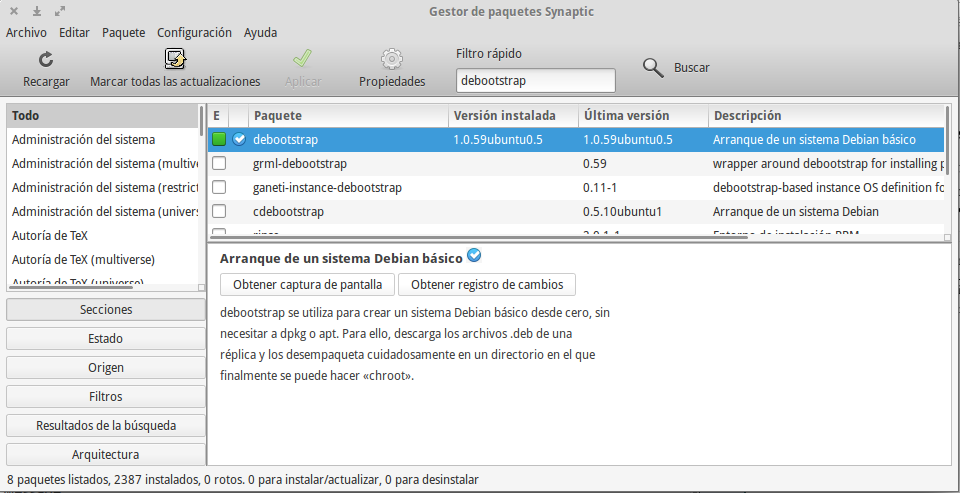
\includegraphics[width=0.9\linewidth]{Figures/QEMU/Synaptic_DBS}}
\caption{Deboostrap dentro de los repositorios.}
\label{fig:DBSRep}
\end{figure}

Utilizando Ubuntu como sistema host, las herramientas ya mencionadas pueden ser encontradas dentro de los repositorios oficiales del sistema, como se muestra en la figura \ref{fig:DBSRep}. Pueden ser instalados por consola o por cualquier gestor de paquetes. Se sugiere actualizar los repositorios mediante el comando:

\begin{lstlisting}[language=bash]
$ sudo apt-get update

\end{lstlisting}
Una vez actualizados, se procede a la instalación de los repositorios:

\begin{lstlisting}[language=bash]
$ sudo apt-get install debootstrap qemu-user-static
\end{lstlisting}

El proceso durará dependiendo de la velocidad de descarga del internet. Al finalizar, se deberá solicitar permiso de \textit{root} al sistema:

\begin{lstlisting}[language=bash]
$ sudo -s
\end{lstlisting}

Ahora, se deberá crear el directorio donde se almacenarán los archivos del sistema que se emulará. Se sugiere que el nombre de dicha carpeta haga referencia al tipo de sistema que contendrá. En este caso, se usará el nombre \textit{ARM-Root}.

\begin{lstlisting}[language=bash]
$ mkdir ~/ARM-Root
\end{lstlisting}

Al finalizar, se procederá a la instalación del sistema:

\begin{lstlisting}[language=bash]
$ debootstrap --foreign --arch=armhf stable ARM-Root
$ cp /usr/bin/qemu-arm-static ARM-Root/usr/bin
$ chroot ARM-Root /debootstrap/debootstrap --second-stage
\end{lstlisting}

El proceso tardará nuevamente dependiendo de la velocidad del internet. Se sugiere estar pendiente del proceso de descarga e instalación por cualquier error que surgiera durante el mismo\footnotemark.

\footnotetext{En ocasiones, suelen salir mensajes de que el archivo a descargar no se encuentra ya en el servidor, pero que lo intentará en otro servidor espejo. Es un mensaje normal y no requiere de la atención del usuario.}

Al finalizar, salga del modo \textit{root} con :

\begin{lstlisting}[language=bash]
$ exit
\end{lstlisting}

Ya dispone de un sistema Debian ARM totalmente funcional, pudiendo acceder mediante el comando:

\begin{lstlisting}[language=bash]
$ sudo chroot ~/ARM-Root /bin/bash
\end{lstlisting}
%---------------------------------------------------

\subsection{Configuración del sistema}\label{subsec:_conf}

Se abre una terminal. En ella, ingrese los comandos para acceder al sistema ARM:

\begin{lstlisting}[language=bash]
$ sudo chroot ~/ARM-Root /bin/bash
\end{lstlisting}

\begin{figure}[H] % Example image
\center{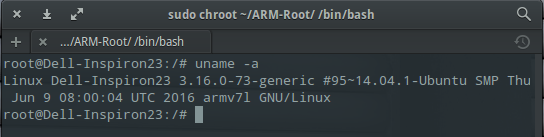
\includegraphics[width=0.9\linewidth]{Figures/QEMU/uname}}
\caption{Salida del comando uname.}
\label{fig:unameout}
\end{figure}

La terminal se debe mostrar como un usuario root dentro del mismo equipo que usted utiliza. Sin embargo, es un sistema de diferente arquitectura. Escriba el siguiente comando para corroborarlo:

\begin{lstlisting}[language=bash]
$ uname -a
\end{lstlisting}

El sistema entregará una salida que contiene el nombre del equipo, versión del kernel, entre otros. Lo interesante está en la salida del tipo de arquitectura del sistema, que dice \textit{armv7l}, como se muestra en la figura \ref{fig:unameout}, lo que indica que la instalación fue exitosa. En la ejecución de una terminal común, sin haber ejecutado el comando \textit{chroot}, la salida ofrecerá en el apartado de arquitectura, a \textit{x86\_64} ó \textit{x86}, dependiendo del sistema anfitrión.

Ahora, conviene actualizar este sistema ARM e instalar los repositorios necesarios que se van a utilizar en el proyecto actual en la tarjeta ARM física original. Para hacer esto, se verifica la versión de Debian instalada mediante el comando:

\begin{lstlisting}[language=bash]
$ cat /etc/debian_version 
\end{lstlisting}

\begin{figure}[H] % Example image
\center{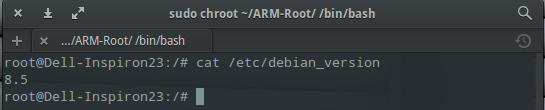
\includegraphics[width=0.9\linewidth]{Figures/QEMU/deb_ver}}
\caption{Versión del sistema instalado.}
\label{fig:debVer}
\end{figure}

Teniendo el número de versión, se debe conocer con qué nombre fue "bautizada" dicha versión de la distribución. Durante la escritura de este documento, la versión instalada fue Debian \textit{Jessie} (versión 8.*), como se muestra en la figura \ref{fig:debVer}. El archivo \textit{/etc/apt/sources.list} es un archivo vacío y en su contenido se debe indicar las direcciones en donde debe buscar por paquetes. Es dependiente de la versión instalada.

En la web  \href{https://linuxconfig.org/debian-apt-get-jessie-sources-list}{LinuxConfig.org\footnotemark} se encuentran listadas las entradas para este archivo en Debian Jessie.

\footnotetext{https://linuxconfig.org/debian-apt-get-jessie-sources-list}

Para este caso particular, se colocarán las entradas para las actualizaciones de seguridad, y del espejo mexicano. Se hace mediante la entrada del comando:

\begin{lstlisting}[language=bash]
$ nano /etc/apt/sources.list
\end{lstlisting}

\begin{figure}[H] % Example image
\center{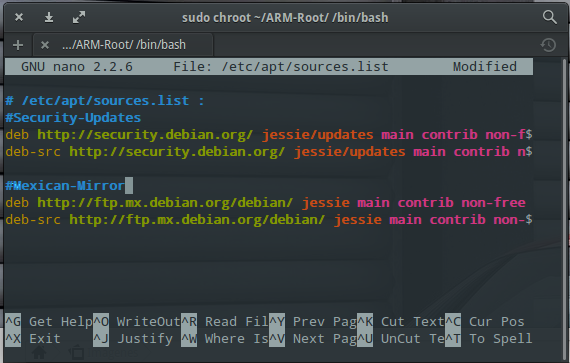
\includegraphics[width=0.9\linewidth]{Figures/QEMU/sources}}
\caption{Contenido del archivo \textit{/etc/apt/sources.list}.}
\label{fig:sources}
\end{figure}

Se vuelve a enfatizar que el contenido de este archivo es totalmente dependiente de la versión de Debian instalada, ya que colocar las fuentes para un sistema diferente puede comprometer el sistema de paquetes de Debian. Una vez colocadas las entradas como muestra la figura \ref{fig:sources}, se procede a actualizar la lista de repositorios mediante el comando:

\begin{lstlisting}[language=bash]
$ apt-get update
\end{lstlisting}

El proceso puede tardar dependiendo de la cantidad de cosas a descargar y de la velocidad a internet. Una vez terminado, se procede a la instalación de los paquetes necesarios para el proyecto en el que se tenga que utilizar este sistema. 

\subsection{Ejemplo: compilando un programa en C++}
Para instalar los compiladores de c y c++, se usa el comando:

\begin{lstlisting}[language=bash]
$ apt-get install build-essential
\end{lstlisting}

El sistema mostrará la cantidad de bytes a descargar y pregunta si se desea proseguir. Con la tecla y/Y se le indica que continúe y mostrará la descarga. Al acabar, el sistema ya será capaz de compilar programas en los lenguajes ya mencionados.

\begin{figure}[H] % Example image
\center{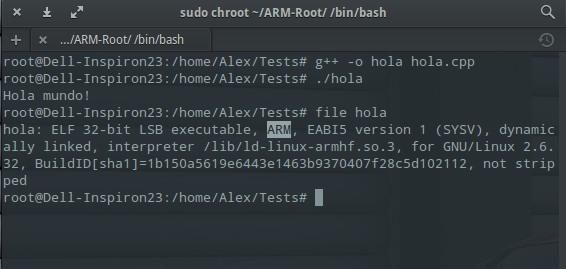
\includegraphics[width=0.9\linewidth]{Figures/QEMU/hola}}
\caption{Compilación, ejecución y verificación de la arquitectura en que fue compilado un programa de c++.}
\label{fig:hola}
\end{figure}

A modo de prueba, se codificó un archivo en c++ que imprima \textit{Hola mundo}, llamado \textit{hola.cpp} y se procedió a compilarlo y ejecutarlo:

\begin{lstlisting}[language=bash]
$ g++ -o hola hola.cpp
$ ./hola
\end{lstlisting}

\newpage

Mediante el comando \textit{file}\footnotemark, se procedió a verificar que el archivo estaba codificado para arquitectura ARM, como indica la figura \ref{fig:hola}. Esto significa que el ejecutable \textit{hola} puede ser ejecutado perfectamente en una tarjeta BeagleBone, Raspberry o similares, de arquitectura ARM con sistema GNU/Linux. Como nota, este archivo no podrá ser ejecutado por una terminal de la computadora host sin haber ejecutado el comando \textit{chroot} mencionado al principio de la subsección \ref{subsec:_conf}, en la página \pageref{subsec:_conf}, debido a que su arquitectura no soporta la codificación de dicho archivo.

\footnotetext{ Instalable mediante: \$ apt-get install file }
%\end{document}